\chapter{Lezione 2 - Approccio quantitativo al progetto e all'analisi. Parte 2}

Continuiamo l'argomento dell'approccio quantitativo al progetto e all'analisi, al progetto e all'analisi di architetture di elaborazione.

\FloatBarrier
\begin{figure}[H]
  \centering
  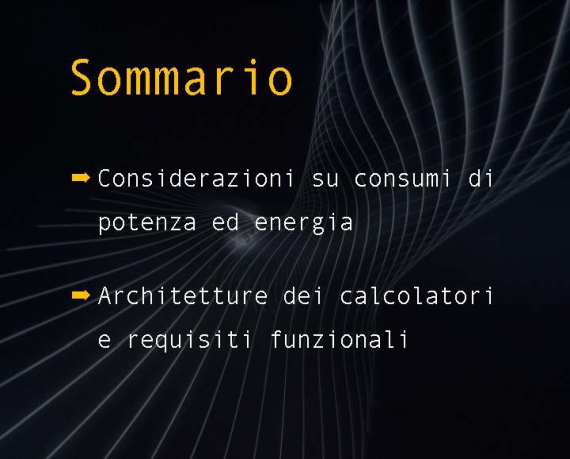
\includegraphics[width=0.40\textwidth,
                    trim=40 80 10 40, % L B R T
                    clip]
                    {images/Lez02_p01_fig_02.png}
  \caption{Sommario}
  \label{fig:Lez02_p01_fig_02}
\end{figure}
\FloatBarrier
\noindent

Il sommario della presente lezione consiste nell'introdurre delle considerazioni su consumi di potenza ed energia, che sono dei fattori molto importanti per i calcolatori e affrontare il problema delle architetture dei calcolatori e dei loro requisiti funzionali.

\section{Consumi di potenza ed energia}

Negli anni questo è diventato uno dei punti più critici delle architetture dei calcolatori.
Per chi è un pochino più giovane, più anziano, ricorderà quando non era sostanzialmente importante in un calcolatore quanto esso consumasse perché il consumo complessivo era generalmente molto inferiore di una piccola lampadina.
Al contrario, negli anni i consumi sono andati via via sempre più aumentando.

\FloatBarrier
\begin{figure}[H]
  \centering
  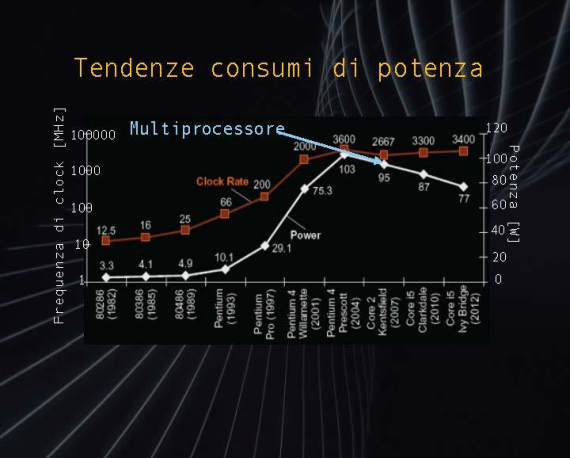
\includegraphics[width=0.8\textwidth,
                    trim=50 110 45 100, % L B R T
                    clip]
                    {images/Lez02_p01_fig_04.png}
  \caption{Consumi di potenza
  \label{fig:Lez02_p01_fig_04}}
\end{figure}
\FloatBarrier
\noindent

E' importante osservare il grafico \ref{fig:Lez02_p01_fig_04} che rappresenta l'andamento dei consumi dell'architettura Intel al variare del tempo.

Consideriamo sull'asse delle ascisse l'architettura Intel 286, che era ancora un'architettura a 16 bit, la prima architettura a 32 bit, il 486 che era un 386 con una unità virgola mobile, poi le prime architetture superscalari, il Pentium, il Pentium Pro e via discorrendo, fino ad arrivare a un picco dei consumi di potenza in corrispondenza delle architetture superscalari. Se ricordate la lezione precedente in corrispondenza di quella accelerazione delle performance dei processori quell'aumento delle prestazioni è venuto sia dalla regge di Moore che dall'aumento del consumo della potenza.

Come vedete negli anni 80 si consumavano poche unità di Watt e a partire dagli anni 90 c'è stata un escalation passando da poche unità di Watt fino a un centinaio di Watt agli inizi degli anni 2000, questi sono dei processori di tipo desktop, alcune architetture server hanno anche raggiunto 150 e più Watt di potenza.

La cosa che è importante osservare è che l'andamento della frequenza di clock è mostrata in scala logaritmica mentre l'evento della potenza è mostrato in una scala lineare, quindi oggettivamente la velocità del processore è aumentata molto più grazie alle leggi di Moore e al contrario la potenza è aumentata ma alla fine di circa un ordine di grandezza e mezzo.

Abbiamo già accennato che attorno a 2003-2004 si è rallentata la corsa dell'aumento delle prestazioni aumentando il paralelismo al livello di istruzioni e hanno cominciato a prendere piedi processori multicore, già qui attorno a 2004-2005 siamo in un ambiente multicore e vi accorgete che il prodotto alto di gamma di desktop Intel in questo caso tende inizialmente addirittura a scendere in velocità e poi più o meno a livellare attorno a 3,4 GHz.

Questo è però negli anni stata accompagnata a una riduzione complessiva del consumo.
Notate che il consumo è uno dei parametri più importanti sia perché se volete utilizzare un apparecchio portatile la potenza deve essere da qualche parte fornita, in questo caso di processori per architetture desktop la maggior problematica è quella della dissipazione della potenza perché questa potenza se viene dissipata deve essere anche smaltita fuori dal processore.

Notate che la legge di Moore comporta che a parità di numero dei gate l'aria scala sostanzialmente come il quadrato e quindi se non diminuisce anche la potenza contemporaneamente il processore verrebbe a scaldarsi in maniera esagerata e prima o poi arrompersi in modo catastrofico.

Quindi il fatto molto importante è osservare che con l'inversione della tendenza da aumento del paralelismo a livello di istruzioni passando alle architetture multicore si è anche cercato di ovviare al problema del continuo aumento della potenza dissipata dal singolo processore in particolare da quello che chiamiamo package.
Nella maggior parte dei casi che noi consideriamo abbiamo un multicore come singolo die, cioè singola lastrina di silicio all'interno di un package.
Esistono delle applicazioni per architetture server o di calcolo parallelo di cui spesso si è fatta avanti la IBM in cui ci sono più chip all'interno del singolo package.
Di questo non parliamo in questo istante e ce ne potremmo occupare forse un pochino più avanti.
Notate, vi ho detto, come i punti di inflessione della curva in parte corrispondono all'avvento delle architetture multicore.

\FloatBarrier
\begin{figure}[H]
  \centering
  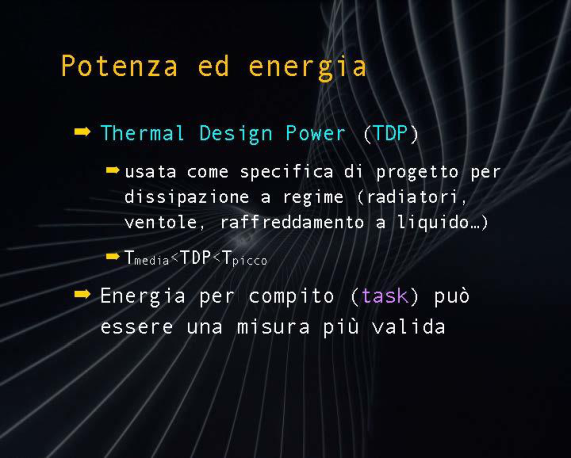
\includegraphics[width=0.6\textwidth,
                    trim=50 110 45 100, % L B R T
                    clip]{images/Lez02_p01_fig_05.png}
  \caption{Thermal design power (TDP)}
  \label{fig:Lez02_p01_fig_05}
\end{figure}
\FloatBarrier
\noindent

Allora, è importante però osservare quali sono i parametri che ci interessano dal punto di vista del progetto di un'architettura di elaborazione. figura \ref{fig:Lez02_p01_fig_05}.

Quello che spesso troverete scritto è il cosiddetto thermal design power o TDP.
Questa grandezza è usata come specifica di progetto per dimensionare il progetto di dissipazione a regime, in particolare l'uso di radiatori, di ventole o eventualmente di raffreddamento al liquido.
Questo è un parametro che trovate quasi sempre e oramai i processori vengono venduti specificando qual è il thermal design power, cioè la potenza che voi dovete rimuovere a regime dal package del vostro processore anche se lo zoccolo stesso contribuisce attraverso la piadinatura a dissipare parte della potenza.
In generale il TDP è compreso fra la potenza media del processore e la potenza di picco, notate che non è nell'uno, nell'altro nella generalità perché la potenza media presuppone un funzionamento generalmente non costante sono pochi casi, in genere quelli di number crunching, di calcolo numerico intenso in cui il processore lavora in continuazione, in molte situazioni, soprattutto negli utilizzi da desktop è molto raro che il processore lavori sul carico massimo per un tempo lunghissimo.

Al contrario a volte il processore può assorbire una potenza elettrica più alta della potenza dissipabile a regime e questo avviene in particolare se le temperature interne, quelle delle giunzioni, sono ancora sufficientemente basse da consentire di accumulare parte del calore in cui l'energia elettrica è stata trasformata e smaltirlo successivamente, quindi immaginate di partire con un processore a temperatura ambiente se la temperatura massima è per esempio 50° facciamo una sia molto conservativa in realtà è un po' più alta, è chiaro che finché la temperatura delle giunzioni non ha raggiunto il punto critico la potenza dissipata può essere maggiore di quella che i dissipatori consentono di dissipare, è chiaro che la maggior potenza elettrica dissipata comporta un aumento della temperatura del processore fino a che si raggiunge una temperatura critica a quel punto la dissipazione deve diminuire perché altrimenti ci potrebbero essere dei danni catastrofici nell'architettura.

Molte volte è però più importante considerare anche l'energia per singolo compito, questa può essere una misura ben più valida, immaginate  dover fare delle transazioni Facebook, Amazon, Google, per ogni transazione che voi fate il tempo di reazione non è critico, deve essere rapido perché l'utente non vuole stare ad aspettare, però se la transazione avviene in un millisecondo o due millisecondi dal punto di vista dell'utente è del tutto irrilevante, dal punto di vista dell'operatore delle architetture che compiono la transazione invece la dissipazione di potenza può essere particolarmente importante, in particolare all'azienda che fornisce quel servizio interessa sapere quant'è l'energia per singola transazione, per esempio ogni volta che voi fate un search su Google sapere quel è un'energia dissipata, sembra strano ma è un'energia abbastanza importante, chi gestisce quel tipo di macchina non si preoccupa tanto di quanto sia la potenza ma quanto sia l'energia per la singola transazione.
Consideriamo altri parametri che ci interessano per analizzare il problema figura \ref{fig:Lez02_p01_fig_06}.

\FloatBarrier
\begin{figure}[H]
  \centering
  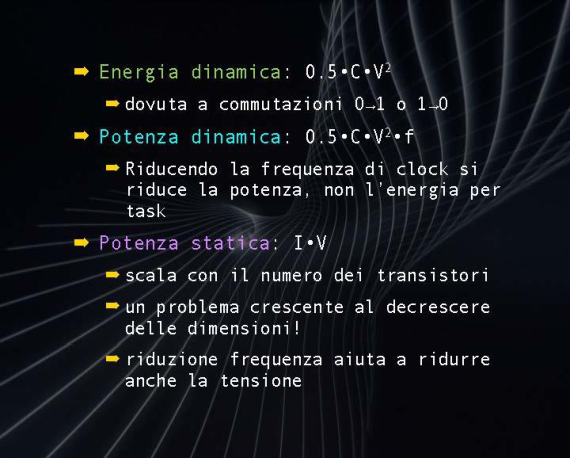
\includegraphics[width=0.6\textwidth,
                    trim=50 50 45 40, % L B R T
                    clip]{images/Lez02_p01_fig_06.png}
  \caption{Energia dinamica, Potenza dinamica, Potenza statica}
  \label{fig:Lez02_p01_fig_06}
\end{figure}
\FloatBarrier
\noindent

dell'energia dinamica che è calcolata come un mezzo della capacità per la tensione di carica a cui viene caricata la capacità stessa, questa è la tipica energia che serve per caricare una porta logica, una capacità C, non sarà una capacità del tutto lineare ma nella nostra approssimazione possiamo considerare una buona approssimazione e in generale la capacità massima a cui viene caricata, se per esempio V è la tensione di pilotaggio dei nostri transistori, questa energia dinamica per il singolo evento di commutazione della singola porta è calcolata come la metà della capacità per la tensione al quadrato.
Sembra un conto molto semplice ma considerate che vi saranno qualche unità di miliardo di transistori e tutto questo concorre all'evento carica delle capacità dei transistori.
In ogni commutazione questa capacità verrà caricata o scaricata e quindi vi sarà una dissipazione di energia.
Al contrario consideriamo come potenza dinamica l'energia moltiplicata per la frequenza di commutazione, se a un singolo evento corrispondono x joule di energia, se andate a 1 GHz di frequenza avrete n joule per 1 GHz e avrete quindi la potenza dinamica necessaria al caricamento delle capacità parassite delle vostre porte. Per molti anni e fino a che non si è avuto uno scaling attorno ai 130 nanometri delle dimensioni di disegno, questa era la potenza più critica nel progetto di un processore.
In generale vi accorgete che riducendo la frequenza di clock si riduce la potenza, non l'energia per task, cioè per compito svolto.
A titolo di esempio se per svolgere un search, ad esempio su Google, occorre svolgere un certo numero di istruzioni, vi accorgete che è irrilevante a che frequenza va il processore, se andasse più lento o più veloce il numero delle istruzioni rimarrebbe uguale e quindi dal punto di vista della potenza dinamica, cioè caricare e scaricare i condensatori nulla cambierebbe.
Come vi ho detto per molti anni la potenza dinamica è stata il parametro più importante di disegno.
Allo scalare delle dimensioni dei transistor sono state anche ridotti gli spessori degli ossidi, i canali sono diventati più corti e quindi ci sono state sempre più correnti di perdita, questo MOS spesso chiamato insulated gate field effect transistor, cioè transistore effetto di campo a porta isolata è diventato sempre meno a porta isolata e quindi cominciava a scorrere corrente dalla giunzione MOS stessa, cominciavano a scorrere anche delle correnti fra source e drain del transistore, al punto tale che diventa importante considerare anche la potenza statica data dal prodotto della corrente per la tensione di alimentazione dei transistor, in genere nei processori la tensione di alimentazione è oggigiorno circa 1 V.
% 12:47
La cosa importante da osservare è che la potenza statica scala con il numero dei transistori, ma non è invariante rispetto alle transazioni perché a parità di tensione di alimentazione più tempo si sta maggiore è l'energia dissipata senza fare nulla di particolare.
La cosa importante è osservare che è un problema crescente al decrescere delle dimensioni dei transistori.
In generale è vero che la potenza statica non varia con la frequenza, però la riduzione della frequenza aiuta anche a ridurre la tensione di alimentazione e quindi indirettamente anche a ridurre la potenza statica.
Vi accorgete che il progetto di un'architettura diventa quindi un fatto sempre più complicato e anche le scelte non solo di progetto del processore ma anche del suo utilizzo in condizioni applicative fa sì che a volte bisogna fare delle scelte, delle scelte di progetto, delle scelte a volte di compromesso, spesso si cerca di fare delle scelte che possano essere flessibili rispetto alle variazioni delle necessità stesse ed questo di cui ci occupiamo in questa lezione e nella successiva.

\section{Tecniche per ridurre i consumi di potenza}

\FloatBarrier
\begin{figure}[H]
  \centering
  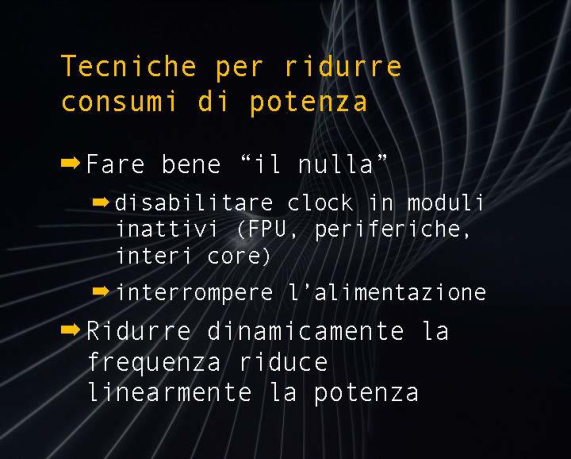
\includegraphics[width=0.6\textwidth,
                    trim=40 40 45 40, % L B R T
                    clip]{images/Lez02_p02_fig_01.png}
  \caption{Tecniche per ridurre i consumi di potenza}
  \label{fig:Lez02_p02_fig_01}
\end{figure}
\FloatBarrier
\noindent

Consigliamo delle tecniche per ridurre i consumi di potenza fig. \ref{fig:Lez02_p02_fig_01}

%15:48
Il primo caso è sempre quello di fare bene il nulla.
Cosa intendo per fare bene il nulla? In molti casi un processore deve fare delle funzioni e a un certo punto smette di farle perché ha finito di fare il compito. Immaginate il vostro telefonino che è un'architettura di elaborazione.
Il vostro telefonino può passare da picchi di carico molto importanti come una compressione video a situazioni dove non fa praticamente niente, l'avete lasciato lì bello sul tavolo e ad esempio avete disabilitato la parte radio quindi il telefono non deve neanche andare a inseguire il segnale, legge un orologio e aggiorna l'orologio e quindi consumerebbe veramente poco.
Quindi quello che è importante è che il vostro telefono nei momenti in cui non è chiamato a fare compressione video, compressione audio, decodifica video, decodifica audio o altre funzionalità per esempio navigare su internet o comunque tutti gli algoritmi di criptografia che ci sono dietro la trasmissione cellulare, è importante che sappia bene fare bene il nulla, cioè consumare poco a riposo.

Per fare questo spesso fra le varie funzionalità si disabilita il clock in moduli inattivi, per esempio nella floating point unit, nell'unità a virgola mobile, in alcune periferiche o addirittura in interi core.
L'esempio è caratteristico, se voi dovete semplicemente aspettare con il vostro sistema, il vostro telefonino, il vostro calcolatore embedded o il vostro desktop di tanto in tanto una comunicazione attraverso una porta esterna, in quel caso l'unità a virgola mobile verosimilmente non dovrà essere utilizzata, bisognerà semplicemente gestire un po' di interrupt dall'esterno per cui l'unità aritmetica e logica e l'unità di controllo bastano e avanzano, quindi l'unità a virgola mobile potrà essere disattivata.
Il primo livello di disattivazione è quello di non far passare il clock, il quale per sua natura determina una potenza dinamica, come vi ho detto nelle slide precedenti, importante perché quelle capacità dovranno essere caricate e scaricate a ogni transizione del clock.

Inoltre è possibile anche interrompere completamente l'alimentazione dai moduli che non occorrono.

Infine si può giocare riducendo dinamicamente la frequenza e ridurre dinamicamente la frequenza consente di ridurre linearmente la potenza dissipata in base alle formule che vi ho dato prima.

Questo gioco dell'interruzione dell'alimentazione in linea di principio non viene a costo zero, nel senso che bisogna dimensionare opportunamente dei transistori come degli interruttori complessivi dell'alimentazione, quindi l'implementazione fisica diventa un po' più complessa, molte volte è vantaggiosa, altre volte non viene utilizzata, oppure viene utilizzata in certe particolari condizioni.
Perché?

Perché notate che dover ridistribuire la potenza comporta quindi comunque dei tempi, ad esempio una maggiore o minore carica di alcuni condensatori, ad esempio quelli di blocco, quindi questo in generale richiede un po' più di impegno sia in termini di tipo progettuale che di gestione del software, perché un'unità a cui è stata interrotta la potenza ci rimette un po' di più a riattivarsi, un'unità a cui è stata o semplicemente disabilitato il clock, ci mette molto di più di un'unità a cui non è stato per niente disabilitato il clock, la quale risponde al prossimo ciclo di clock come qualunque macchina sequenziale.

In ultima riga vi ho detto anche che si provvede a ridurre dinamicamente la frequenza e in realtà il risparmio di potenza è più che lineare, nel caso si riduca la frequenza, perché come vi ho già accennato, ridurre la frequenza può consentire anche di ridurre la tensione di alimentazione che a sua volta riduce sia la potenza statica che la potenza dinamica ed è quello che spesso avviene nella maggioranza dei processori, sia desktop che per applicazioni portati dove la potenza è importante sia in termini di disponibilità di energia nelle batterie, sia in termini di dissipazione della potenza stessa, perché ad esempio nessuno di noi vorrebbe una voluminosa ventola montata sul nostro bellissimo telefonino o nel nostro bellissimo smartphone.

\FloatBarrier
\begin{figure}[H]
  \centering
  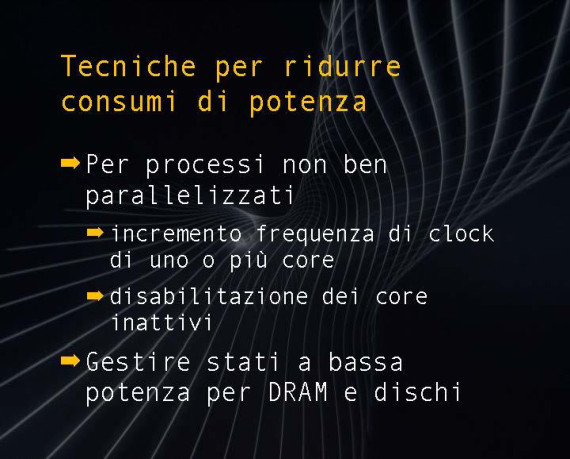
\includegraphics[width=0.6\textwidth,
                    trim=40 40 45 40, % L B R T
                    clip]{images/Lez02_p02_fig_02.png}
  \caption{Altre tecniche per ridurre i consumi di potenza}
  \label{fig:Lez02_p02_fig_02}
\end{figure}
\FloatBarrier
\noindent

Vediamo (fig. \ref{fig:Lez02_p02_fig_02}) altre tecniche per ridurre i consumi di potenza per processi ad esempio non ben parallelizzati, si procede all'incremento di frequenza di clock di 1 o più core e contemporaneamente si disabilitano i core inattivi.
Questo ragionamento sembra essere in contrasto con quello che vi ho detto, cioè con la tendenza di avere sempre più core e una frequenza decrescente, ma considerate che non tutti i processi sono facilmente parallelizzabili o semplicemente sono dei processi che sono stati scompilati anni prima senza tener conto dell'esistenza di più core e quindi non sono più parallelizzabili e avete soltanto il codice macchina.
Quindi in quei casi se volete effettivamente avere una migliore efficienza, cioè maggiori prestazioni e minori consumi, non vi resta altro che spegnere i core non utilizzati perché non utilizzabili da quel codice e aumentare nei limiti del possibile la frequenza dei core in uso.

Infine è utile gestire stati a bassa potenza sia per le dram che per i dischi, quindi i dischi magnetici vengono messi ad esempio con le testine in parcheggio, cioè il disco viene fermato e così risparmiate qualche Watt di potenza.

Vi do adesso uno spunto per la riflessione e vi invito a riflettere per le diverse classi di calcolatori elencando cause e criticità della dissipazione di potenza.
Ovviamente torneremo su questo avanti nel corso ma è importante che voi vi fermiate un attimo, cerchiate di riflettere su quali possono essere le cause soprattutto quali siano le criticità nelle diverse classi di calcolatori che conoscete o che venite progressivamente a conoscere. Ponetevi sempre queste domande perché non è un dettaglio irrilevante.

\section{Le architetture dei calcolatori e i requisiti funzionali}

\FloatBarrier
\begin{figure}[H]
  \centering
  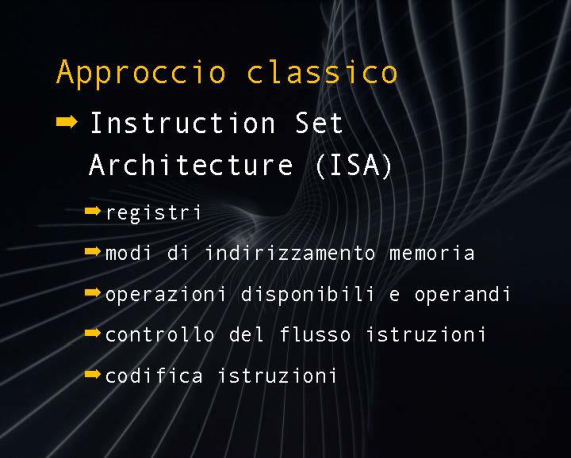
\includegraphics[width=0.6\textwidth,
                    trim=40 40 45 40, % L B R T
                    clip]{images/Lez02_p02_fig_05.png}
  \caption{Architetture dei calcolatori e requisiti funzionali}
  \label{fig:Lez02_p02_fig_05}
\end{figure}
\FloatBarrier
\noindent

Continuiamo con il prossimo argomento, cioè le architetture dei calcolatori e i requisiti funzionali (fig. \ref{fig:Lez02_p02_fig_05}).
L'approccio classico alle architetture dei calcolatori è la cosiddetta instruction set architecture, cioè il repertorio istruzioni dell'architettura ISA.

Tipicamente in una ISA si considerano i registri, i modi di indirizzamento della memoria, le operazioni disponibili nel repertorio e gli operandi, il controllo del flusso di istruzioni e il modo in cui le istruzioni sono codificate, cioè la codifica dell'istruzione all'interno della parola istruzione.
Sempre nell'approccio classico altri aspetti vengono posti in secondo piano e vengono chiamati in modo implicitamente riduttivo implementazione. Questo invece è particolarmente importante.

\FloatBarrier
\begin{figure}[H]
  \centering
  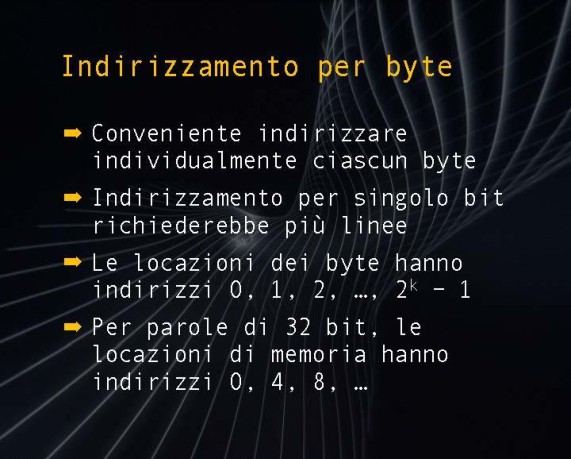
\includegraphics[width=0.6\textwidth,
                    trim=40 40 45 40, % L B R T
                    clip]{images/Lez02_p03_fig_01.png}
  \caption{Indirizzamnto per byte}
  \label{fig:Lez02_p03_fig_01}
\end{figure}
\FloatBarrier
\noindent

\subsection{Indirizzamento a byte}
Consideriamo un esempio fig. \ref{fig:Lez02_p03_fig_01} nelle architetture in cui l'indirizzamento è per byte e risulta conveniente indirizzare individualmente ciascun byte, ma l'indirizzamento del singolo bit non viene fatto perché richiederebbe più linee.
Nell'evoluzione storica dove anche le piste erano importanti ha fatto sì che ci si è stabilizzati come elemento minimo indirizzabile indipendentemente al byte e non al bit e non al nibble.
Questa è una scelta e in alcuni casi uno potrebbe addirittura lavorare direttamente solo sulla parola, in alcune architetture, ad esempio i digital signal processors, questo a volte viene fatto ma non è molto comune.
In generale è importante osservare che si indirizza per byte.
Le locazioni dei byte hanno indirizzi progressivi 0, 1, 2 fino a $2^k-1$ , se k sono il numero delle locazioni.
Per parole di 32 bit le locazioni di memoria hanno sempre indirizzi 0, 4, 8 e così via, cioè multipli di 4.

\textit{0 corrispnde al 1° byte, 1 al 2° byte, ... su 4 byte avrò 4*8=32 bit}

\subsection{big-endian, little-endian e bi-endian}

\FloatBarrier
\begin{figure}[H]
  \centering
  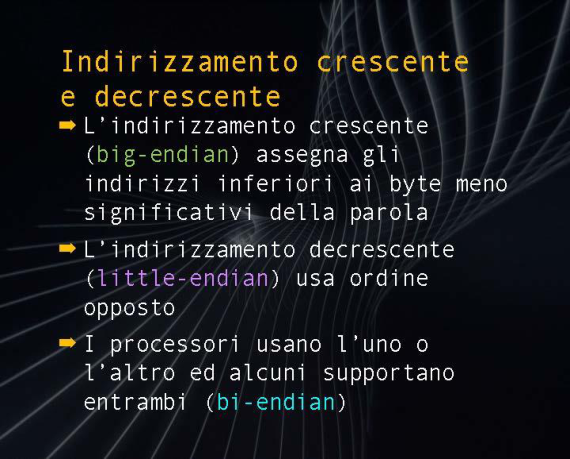
\includegraphics[width=0.6\textwidth,
                    trim=40 40 45 40, % L B R T
                    clip]{images/Lez02_p03_fig_02.png}
  \caption{big-endian, little-endian e bi-endian}
  \label{fig:Lez02_p03_fig_02}
\end{figure}
\FloatBarrier
\noindent

Consideriamo quello che viene chiamato indirizzamento crescente o indirizzamento decrescente (fig. \ref{fig:Lez02_p03_fig_02}).
Si dice indirizzamento crescente o big-endian in inglese quello che assegna gli indirizzi inferiori ai byte meno significativi della parola. L'indirizzo decrescente o little-endian usa l'ordine opposto.
Alcuni processori usano o l'uno o l'altro ma in alcuni particolari i processori sono anche supportati entrambi i modi, in quel caso i processori vengono detti bi-endian.
La scelta della modalità dell'indirizzamento crescente o decrescente, little-endian o big-endian in questi processori viene fatto spesso esclusivamente in fase di avvio mediante il controllo per esempio di un apposito piedino che  consente al processore di interpretare correttamente gli indirizzi.
La definizione non è così intuitiva, un esempio è la cosa più semplice.

\FloatBarrier
\begin{figure}[H]
  \centering
  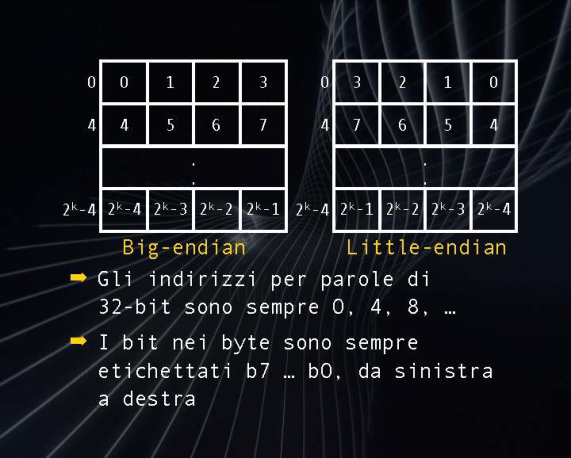
\includegraphics[width=0.6\textwidth,
                    trim=40 40 45 40, % L B R T
                    clip]{images/Lez02_p03_fig_03.png}
  \caption{big-endian, little-endian e bi-endian}
  \label{fig:Lez02_p03_fig_03}
\end{figure}
\FloatBarrier
\noindent

Considerate una parola di 32 bit (fig. \ref{fig:Lez02_p03_fig_03}), 4 byte, nel caso del big-endian e il byte più a sinistra è quello che definisce l'indirizzo della parola, cioè il byte di peso più significativo, al contrario nel caso del little-endian è l'indirizzo del byte meno significativo, cioè del little, del piccolo, che definisce l'indirizzo della parola.
La parola successiva sarà, se la prima è a 0, la seconda sarà 4, che corrisponde ancora all'indirizzo del byte meno significativo.

Questo è utile da sapere perché spesso molti software, molti codici, i dati vengono memorizzati per semplificare il processamento dei byte.
Se andate a vedere la codifica di alcuni algoritmi di compressione video o di immagine, questo viene messo, ad esempio il TIFF è uno tipico di questo in cui voi potete scegliere l'ordinamento dei byte che rappresentano le parole, l'indirizzo dei file. Questo perché alcuni architettore leggono più facilmente una modalità invece che l'altra.

Gli indirizzi per parole di 32 bit però sono sempre a 0, 4 o 8, quindi indipendentemente da fatto che siano big-endian o little-endian, l'indirizzo è sempre a multipli di 4.
Quello che cambia è l'indirizzamento dei byte della parola rispetto ai byte e il modo in cui questi possano essere più rapidamente gestiti del processore o dove si debba agire sul singolo byte.
I bit nei byte sono sempre etichettati b7, b0 da sinistra a destra, quindi indipendentemente da tutto all'interno di un byte l'ordine è sempre lo stesso.

\subsection{Allineamento di parola} 

\FloatBarrier
\begin{figure}[H]
  \centering
  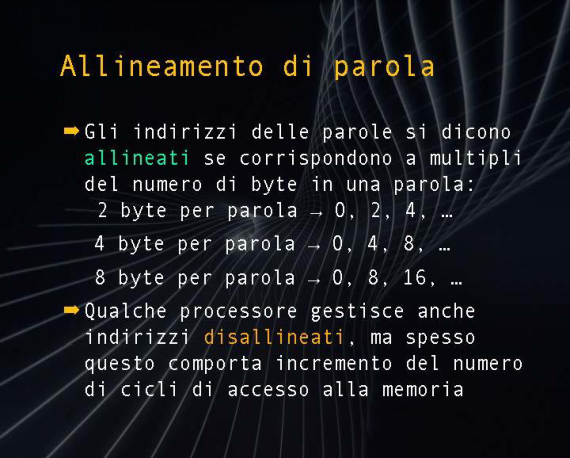
\includegraphics[width=0.6\textwidth,
                    trim=40 40 45 40, % L B R T
                    clip]{images/Lez02_p03_fig_04.png}
  \caption{Allineamento di parola}
  \label{fig:Lez02_p03_fig_04}
\end{figure}
\FloatBarrier
\noindent

Consideriamo quello che viene chiamato allineamento di parola (fig. \ref{fig:Lez02_p03_fig_04}).

Gli indirizzi delle parole si dicono allineati se corrispondono a multipli del numero di byte in una parola.
Ad esempio se una parola è fatta di 2 byte gli indirizzi sono 0, 2 o 4, se 4 byte 0, 4 o 8, se di 8 byte come ad esempio in un double precision floating point, 0, 8, 16 e così via.
Qualche processore gestisce anche indirizzi disallineati, ma spesso questo comporta incremento del numero dei cicli di accesso alla memoria.
Tipicamente alcune architetture ad esempio l'ARM consente l'accesso disallineato di 2 byte, cioè alla mezza parola, questo però non è che viene a costo 0, viene al costo di un ciclo di clock in più, cioè c'è un buffer di riordino interno che consente di accedere anche alle mezze parole.
Il motivo per cui l'ARM consente anche l'utilizzo di 16 bit verrà chiarito più avanti nel corso delle lezioni.

\subsection{Confronto tra SISC e RISC}

\FloatBarrier
\begin{figure}[H]
  \centering
  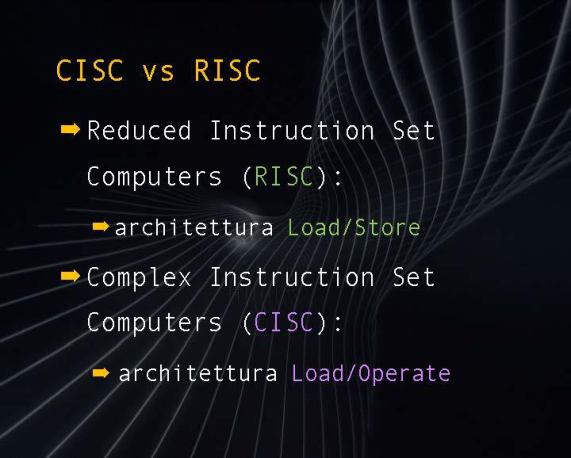
\includegraphics[width=0.6\textwidth,
                    trim=40 40 45 40, % L B R T
                    clip]{images/Lez02_p03_fig_05.png}
  \caption{Confronto tra SISC e RISC}
  \label{fig:Lez02_p03_fig_05}
\end{figure}
\FloatBarrier
\noindent
 

Vediamo il confronto tra i cosiddetti SISC e RISC (fig. \ref{fig:Lez02_p03_fig_05}).

RISC sta per Reduced Instruction Set Computer ed è un'architettura caratterizzata dall'essere load store.
Non importa quante sono le istruzioni, se le istruzioni sono semplici o complesse, semplici e complesse sono delle definizioni più diciamo filosofice che sostanziali, quello che conta è l'architettura load store, cioè l'unica operazione che sulla memoria sono operazioni di caricamento di immagazzinamento, agiscono solo su registri.

Al confronto le cosiddette architetture SISC sono delle architetture di tipo load operator, cioè sono possibili operazioni direttamente sugli operandi in memoria, quindi queste agiscono sia su registri che su memoria.

\FloatBarrier
\begin{figure}[H]
  \centering
  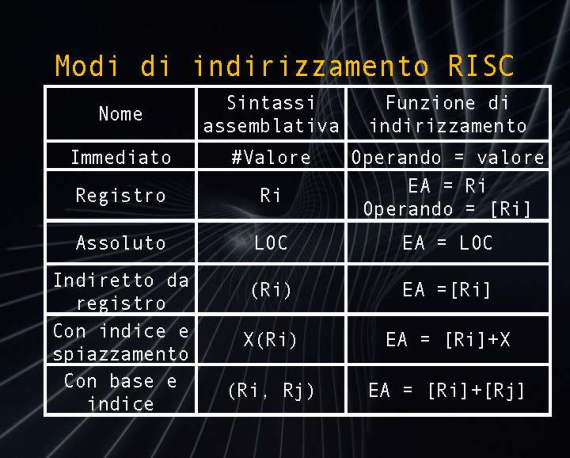
\includegraphics[width=0.6\textwidth,
                    trim=40 40 45 40, % L B R T
                    clip]{images/Lez02_p03_fig_06.png}
  \caption{Modi indirizzamento RISC}
  \label{fig:Lez02_p03_fig_06}
\end{figure}
\FloatBarrier
\noindent

I modi di indirizzamento dei RISC, quelli più comuni e quelli sempre esistenti sono:

\begin{itemize}
  \item il modo immediato in cui la sintassi assemblativa si dà direttamente il valore, l'operando e il valore segnato nel campo
  \item Il modo registro in cui la sintassi assemblativa vi dà il valore di un registro e l'indirizzo effettivo, l'effective address in inglese, è dato dal registro stesso.
  \item Il modo assoluto è dato da una locazione in memoria, cioè l'indirizzo effettivo è dato dal contenuto della locazione in memoria
  \item Indirizzamento diretto da registro; nella sintassi assemblativa in alcuni casi si usano le parentesi tonde per rappresentare Ri e l'indirizzo viene pescato in un registro e quindi il contenuto di quel registro diventa l'indirizzo effettivo
  \item E' possibile anche un modo indice e spiazzamento in cui X è lo spiazzamento, Ri è l'indirizzo efficace e dato dal contenuto di Ri più il valore dello spiazzamento che è una costante X.
  \item registro base e registro indice, l'indirizzo effettivo è dato dalla somma dei contenuti dei due registri.
\end{itemize}


Esistono anche delle variazioni in cui si può mettere uno spiazzamento in aggiunta ai due registri e quindi l'indirizzo  effettivo è la somma dei contenuti dei due registri più lo spiazzamento.

In generale il modo X Ri Rj è quello più generale perché se si mette come X zero si ha il base con indice, se si mette uno dei due registri a zero si ha indice spiazzamento, se si mette uno dei due registri e lo spiazzamento a zero si ha  l'indiretto da registro.
%31:58
\FloatBarrier
\begin{figure}[H]
  \centering
  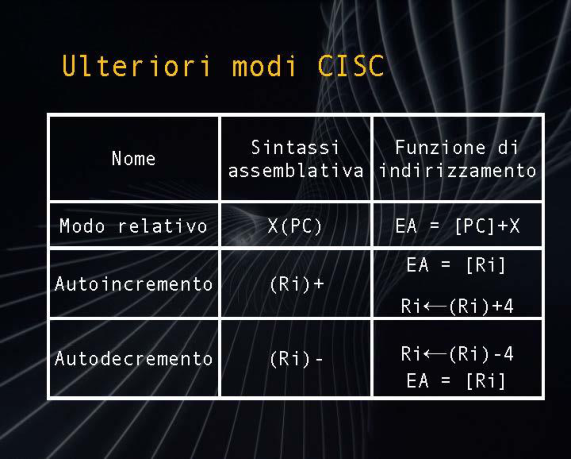
\includegraphics[width=0.6\textwidth,
                    trim=40 40 15 40, % L B R T
                    clip]{images/Lez02_p04_fig_01.png}
  \caption{Modi indirizzamento CISC}
  \label{fig:Lez02_p04_fig_01}
\end{figure}
\FloatBarrier
\noindent

Nel caso dei CISC vi sono anche altri modi di indirizzamento, il modo relativo, in questo caso è il program counter quindi è un modo con indice dove il registro indice non è altro che il program counter.
L'autodecremento e l'autodecremento sono particolarmente interessanti perché in una singola operazione apparentemente il processore è in grado sia di calcolare l'indirizzo effettivo leggendo il contenuto del registro e immediatamente aggiornare il contenuto del registro e aumentandolo di uno.
L'autodecremento è analogo in cui prima si decrementa il contenuto del registro e poi si ottiene il registro.
Notate che queste operazioni non sempre riescono ad avvenire un singolo colpo di clock. 

\subsubsection{Lunghezza fissa e variabile delle istruzioni}

Passiamo a considerare lunghezza fissa e variabile delle istruzioni 

\FloatBarrier
\begin{figure}[H]
  \centering
  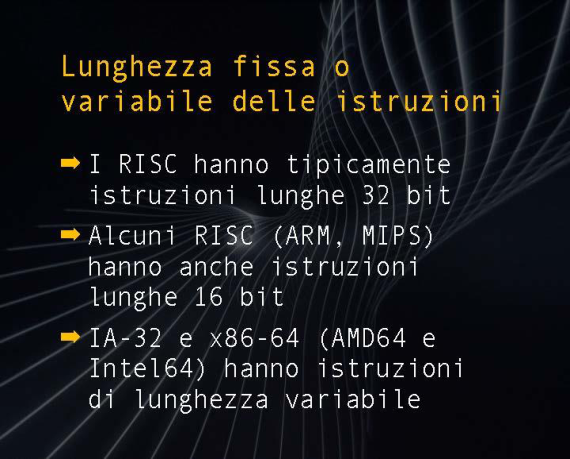
\includegraphics[width=0.6\textwidth,
                    trim=40 40 15 40, % L B R T
                    clip]{images/Lez02_p04_fig_02.png}
  \caption{Lunghezza fissa e variabile delle istruzioni}
  \label{fig:Lez02_p04_fig_02}
\end{figure}
\FloatBarrier
\noindent

Come vi ho detto i RISC hanno tipicamente istruzioni lunghe di 32 bit ma esistono delle situazioni in cui è utile impacchettare istruzioni più piccole.

Perché non facciamo sempre istruzioni più piccole?

Perché le istruzioni più piccole spesso vengono con una penalità.
Per esempio lo vedremo quando tratteremo l'architettura ARM ma come ho detto alcuni RISC come l'ARM e anche lo stesso MIPS hanno la possibilità di utilizzare istruzioni a 16 bit.
Queste istruzioni non sono mischiate nello stesso codice con le istruzioni a 32 bit. Vi sono due stati diversi del processore.
Uno che è in grado di interpretare istruzioni a 32 bit e un altro stato che è in grado di interpretare istruzioni a 16 bit.
Per compiti poco onerosi dal punto di vista computazionale ma dove la quantità di memoria è vincolante si può ricorrere a istruzioni a 16 bit.
Nel caso dell'ARM vengono chiamate TAMB come nome per definirle.

Il caso opposto è quello delle istruzioni di architettura Intel a 32 e 64 bit; nella 64 bit ci sono due diverse implementazioni e hanno istruzioni di lunghezza variabile.
Tipicamente da 1 a 12 byte.
Quindi alcune istruzioni possono essere molto brevi, altre istruzioni possono essere veramente lunghe.
Si usano quelle che vengono chiamate i prefix nelle istruzioni e fanno sì che la decodifica di queste istruzioni sia tutto tranne che elementare come abbiamo visto nel corso del primo livello sull'istruzione di decodifica di una istruzione RISC ma overhead della decodifica delle istruzioni di un repertorio CISC è venuto a perdersi col passare del tempo.

\subsubsection{Approccio holistico}

Consideriamo invece al contrario ora quello che viene chiamato un approccio olistico (fig. \ref{fig:Lez02_p04_fig_03})

\FloatBarrier
\begin{figure}[H]
  \centering
  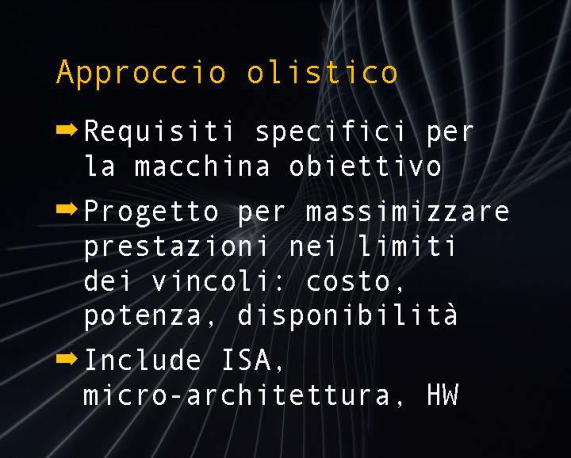
\includegraphics[width=0.6\textwidth,
                    trim=40 40 15 40, % L B R T
                    clip]{images/Lez02_p04_fig_03.png}
  \caption{Apprccio olistico}
  \label{fig:Lez02_p04_fig_03}
\end{figure}
\FloatBarrier
\noindent

Questo approccio non tiene più conto solo dell'architettura e del repertorio istruzioni ma considera i requisiti specifici di una macchina obiettiva. Noi dobbiamo disegnare una macchina, cioè un'architettura di elaborazione che abbia un preciso obiettivo. Deve essere un telefonino cellulare, deve essere un netbook, deve essere un desktop, deve essere una software house, deve essere un supercalcolatore.
Il requisito va preso complessivamente, non è che ci si può limitare al solo repertorio di istruzioni e occorre cercare di fare un progetto per massimizzare le prestazioni e i limiti dei vincoli.
I vincoli possono essere il costo dei componenti, la potenza dissipata, la disponibilità del sistema, cioè quanto questo sistema sia robusto rispetto a problemi.
Per esempio se dovete fare un server di dati vi interesserà che anche se si rompe uno dei dischi il sistema continui ancora a fornire il servizio.
Se avete per esempio il gestore dei bancomat di una banca, capite quanto è importante che la disponibilità sia continua.
Se gestite un portale di vendita e quello che certamente non volete è che vi si rompa il portale di vendita soggetto a sovraccarico nei giorni immediatamente precedenti natale, quando la maggior parte degli acquisti, i regali e quant'altro viene fatto.

All'interno di questo approccio olistico consideriamo tutto, consideriamo anche l'ISA, la microarchitettura con cui questa isa è implementata e alcuni dettagli dell'hardware che andiamo a definire più avanti.

\subsubsection{Organizzazione di un calcolatore}

Cos'è l'organizzazione di un calcolatore?

\FloatBarrier
\begin{figure}[H]
  \centering
  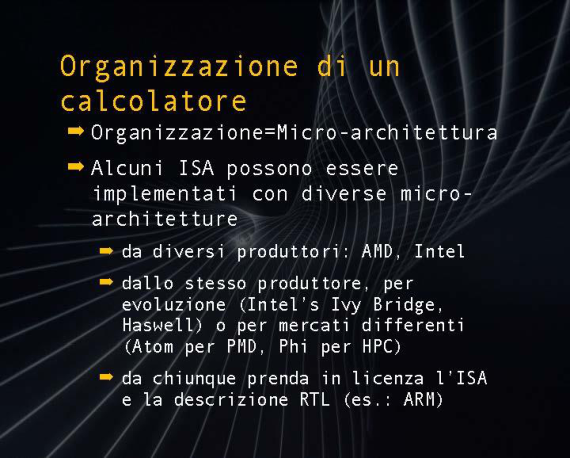
\includegraphics[width=0.6\textwidth,
                    trim=40 40 15 40, % L B R T
                    clip]{images/Lez02_p04_fig_04.png}
  \caption{Apprccio olistico}
  \label{fig:Lez02_p04_fig_04}
\end{figure}
\FloatBarrier
\noindent

A volte trovate il termine organizzazione, altre volte trovate il termine microarchitettura.
Alcune ISA possono essere implementate con diverse microarchitetture, ad esempio possono essere implementate da diversi produttori AMD e Intel, vi ho raccontato come durante la guerra RISC-CISC degli anni 90, a un certo punto AMD ha cominciato a implementare il repertorio di istruzioni Intel trascodificando le istruzioni Intel nelle istruzioni native dei suoi processori.

Similmente ha fatto Intel, ma il modo in cui queste microarchitetture sono state realizzate sono del tutto diverse fra AMD e Intel.
Anche lo stesso produttore, per esempio, Intel ha evoluto le sue microarchitetture, per esempio negli anni in cui vi sto parlando, l'Ivy Bridge e l'Haswell sono due variazioni evolutive della stessa microarchitettura, ma non sono più identiche.
A volte le microarchitetture sono radicalmente diverse pur supportando lo stesso ISA, questo per esempio per differenziare i desktop o i server, nel caso dell'Ivy Bridge e dell'Haswell, dall'ATOM per le applicazioni mobili o dall'Intel Phi per le applicazioni di calcolo ad alte prestazioni, high performance computation.
In generale poi la microarchitettura può essere customizzata da chiunque prende in licenza l'ISA dal proprietario dell'ISA e eventualmente una descrizione register transfer logic.
Questo è quello che avviene tipicamente con ARM, cioè voi pagate una licenza all'azienda ad ARM e acquisite il diritto o ad utilizzare solo l'instruction set architecture o addirittura prendete il register transfer logic description del microprocessore.

\subsubsection{Hardware}

Vediamo cosa si intende per hardware.

\FloatBarrier
\begin{figure}[H]
  \centering
  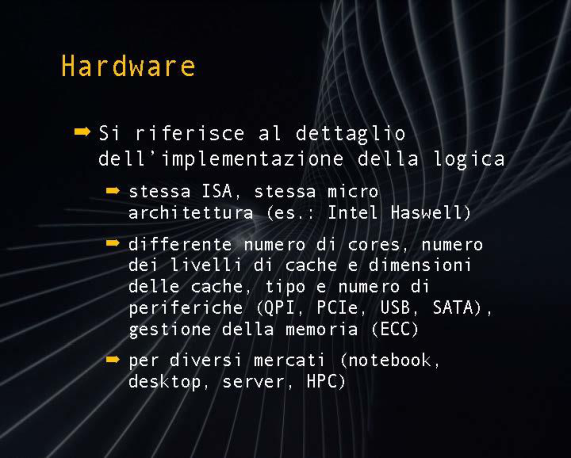
\includegraphics[width=0.6\textwidth,
                    trim=40 40 15 40, % L B R T
                    clip]{images/Lez02_p04_fig_05.png}
  \caption{Hardware}
  \label{fig:Lez02_p04_fig_05}
\end{figure}
\FloatBarrier
\noindent

Si riferisce al dettaglio dell'implementazione della logica, quindi stesso ISA, stesso microarchitettura, ad esempio lo stesso Intel Aswell, ma differente di cores 2, 4, 8, 16, differente numero dei livelli di cache, L1 e L2, a volte anche L3, differente dimensione della cache, numero di periferiche, se via quick pack interconnect, quante porte PCI express, quante porte USB, quante SATA, la gestione della memoria con o senza codici di correzione d'errore.
Questi vengfono utilizzati in diversi mercati notebook, desktop, servers e high performance computing.

Spunto per la riflessione e vi chiedo perché non è sufficiente limitarsi a considerare l'ISA e la frequenza di clock nella valutazione della scelta di un processore.

Quello che molti ragazzi fanno, compro il processore più veloce, prendo il clock più veloce e non me ne preoccupo.
Se volete riflettere su quello che già vi ho detto, apritevi e createvi dei dubbi, li risolveremo in parte nelle lezioni successive, ma è importante voi che vi poniate il dubbio di non ragionare sempre, certamente solo su un solo parametro, il clock più veloce o più core e basta.